%% Aide-mémoire
\documentclass[10pt, french]{article}
%% -----------------------------
%% Préambule
%% -----------------------------
\usepackage{xcolor}
\usepackage{bbding}
\usepackage{pifont}
\usepackage{tikz}
\usepackage{pgfplots}
\usepackage{array}
\definecolor{LongColor}{HTML}{E61D3B}
\definecolor{ShortColor}{HTML}{2C97D8}
\def\cours{Gestion du risque financier II}
\def\sigle{ACT-2011}
\def\session{Hiver 2018}
\def\auteur{Nicholas Langevin}
\def\BackgroundColor{white}
\def\SectionColor{black!30!black}
\def\SubSectionColor{black!30!black}
% !TEX encoding = UTF-8 Unicode
% LaTeX Preamble for cheatsheet
% Author : Gabriel Crépeault-Cauchon

% HOW-TO : copy-paste this file in the same directory as your .tex file, and add in your preamble the next command right after you have specified your documentclass :
% \input{preamble-cheatsht.tex}
% ---------------------------------------------
% ---------------------------------------------

% Extra note : this preamble creates document that are meant to be used inside the multicols environment. See the documentation on internet for further information.

%% -----------------------------
%% Encoding packages
%% -----------------------------
\usepackage[utf8]{inputenc}
\usepackage[T1]{fontenc}
\usepackage{babel}
\usepackage{lmodern}

%% -----------------------------
%% Variable definition (change these values)
%% -----------------------------
\def\cours{Analyse probabiliste des risques actuariels}
\def\sigle{ACT-1002}
\def\session{H2017}
\def\auteur{Gabriel Crépeault-Cauchon}
\def\BackgroundColor{white}
\def\SectionColor{teal!50!black}
\def\SubSectionColor{teal!20!black}

%% -----------------------------
%% Margin and layout
%% -----------------------------
% Determine the margin for cheatsheet
\usepackage[landscape, hmargin=1cm, vmargin=1.7cm]{geometry}
\usepackage{multicol}

% Remove automatic indentation after section/subsection title.
\setlength{\parindent}{0cm}

% Save space in cheatsheet by removing space between align environment and normal text.
\usepackage{etoolbox}
\newcommand{\zerodisplayskips}{%
  \setlength{\abovedisplayskip}{0pt}%
  \setlength{\belowdisplayskip}{0pt}%
  \setlength{\abovedisplayshortskip}{0pt}%
  \setlength{\belowdisplayshortskip}{0pt}}
\appto{\normalsize}{\zerodisplayskips}
\appto{\small}{\zerodisplayskips}
\appto{\footnotesize}{\zerodisplayskips}

%% -----------------------------
%% URL and links
%% -----------------------------
\usepackage{hyperref}
\hypersetup{colorlinks = true, urlcolor = gray!70!white, linkcolor = black}

%% -----------------------------
%% Document policy (uncomment only one)
%% -----------------------------
%	\usepackage{concrete}
	\usepackage{mathpazo}
%	\usepackage{frcursive} %% permet d'écrire en lettres attachées
%	\usepackage{aeguill}
%	\usepackage{mathptmx}
%	\usepackage{fourier}

%% -----------------------------
%% Math configuration
%% -----------------------------
\usepackage[fleqn]{amsmath}
\usepackage{amsthm,amssymb,latexsym,amsfonts}
\usepackage{empheq}
\usepackage{numprint}

% Mathematics shortcut
\newcommand{\reels}{\mathbb{R}}
\newcommand{\entiers}{\mathbb{Z}}
\newcommand{\naturels}{\mathbb{N}}
\newcommand{\eval}{\biggr \rvert}
\usepackage{cancel}
\newcommand{\derivee}[1]{\frac{\partial}{\partial #1}}
\newcommand{\prob}[1]{\Pr \left( #1 \right)}
\newcommand{\esp}[1]{\mathrm{E} \left[ #1 \right]} % espérance
\newcommand{\variance}[1]{\mathrm{Var} \left( #1   \right)}
\newcommand{\covar}[1]{\mathrm{Cov} \left( #1   \right)}
\newcommand{\laplace}{\mathcal{L}}

% To indicate equation number on a specific line in align environment
\newcommand\numberthis{\addtocounter{equation}{1}\tag{\theequation}}

% Actuarial notation package
\usepackage{actuarialsymbol}
\usepackage{actuarialangle}

% Matricial anotation for math symbols (\bm{•})
\usepackage{bm}
% matricial notation variable (bold style)
\newcommand{\matr}[1]{\mathbf{#1}}



%% -----------------------------
%% tcolorbox configuration
%% -----------------------------
\usepackage{tcolorbox}
\tcbuselibrary{xparse}
\tcbuselibrary{breakable}

%% Définition boite pour définition
\DeclareTColorBox{definition}{ o }% #1 parameter
{colframe=blue!60!green,colback=blue!5!white, % color of the box
breakable, pad at break*=0mm, % to split the box
title = {#1},
after title = {\large \hfill \faBook}
}

%% -----------------------------
%% Graphics and pictures
%% -----------------------------
\usepackage{graphicx}
\usepackage{pict2e}

%% -----------------------------
%% insert pdf pages into document
%% -----------------------------
\usepackage{pdfpages}

%% -----------------------------
%% Color configuration
%% -----------------------------
\usepackage{color, soulutf8, colortbl}

% usefull shortcut for colored text
\newcommand{\orange}{\textcolor{orange}}
\newcommand{\red}{\textcolor{red}}
\newcommand{\cyan}{\textcolor{cyan}}
\newcommand{\blue}{\textcolor{blue}}
\newcommand{\green}{\textcolor{green}}
\newcommand{\purple}{\textcolor{magenta}}
\newcommand{\yellow}{\textcolor{yellow}}


%% -----------------------------
%% Enumerate environment configuration
%% -----------------------------
% Custum enumerate & itemize Package
\usepackage{enumitem}
% French Setup for itemize function
\frenchbsetup{StandardItemLabels=true}
% Change default label for itemize
\renewcommand{\labelitemi}{\faAngleRight}

%% -----------------------------
%% Tabular column type configuration
%% -----------------------------
\newcolumntype{C}{>{$}c<{$}} % math-mode version of "l" column type
\newcolumntype{L}{>{$}l<{$}} % math-mode version of "l" column type
\newcolumntype{R}{>{$}r<{$}} % math-mode version of "l" column type
\newcolumntype{f}{>{\columncolor{green!20!white}}p{1cm}}
% configuration to force a line break within a single cell
\usepackage{makecell}



%% -----------------------------
%% Fontawesome for special symbols
%% -----------------------------
\usepackage{fontawesome}

%% -----------------------------
%% Section Font customization
%% -----------------------------
\usepackage{sectsty}
\sectionfont{\color{\SectionColor}}
\subsectionfont{\color{\SubSectionColor}}

%% -----------------------------
%% Footer/Header Customization
%% -----------------------------
\usepackage{lastpage}
\usepackage{fancyhdr}
\usepackage{titling}
\pagestyle{fancy}
% Header
\fancyhead{} 	% Reset
\fancyhead[L]{Aide-mémoire pour~ \cours ~(\textbf{\sigle})}
\fancyhead[R]{\auteur}

% Footer
\fancyfoot{}		% Reset
\fancyfoot[R]{\thepage ~de~ \pageref{LastPage}}
\fancyfoot[L]{\href{https://github.com/gabrielcrepeault/latex-template}{\faGithub \ gabrielcrepeault/latex-template}}

% page background color
\pagecolor{\BackgroundColor}






%% END OF PREAMBLE
% ---------------------------------------------
% ---------------------------------------------

\title{GRF-II \\ Document d'étude}
\author{Nicholas Langevin}
%% -----------------------------
%% Début du document
%% -----------------------------
\begin{document}

% PAGE COUVERTURE DE L'AIDE-MÉMOIRE
\maketitle 
\vspace{50px}
\begin{center}
\begin{minipage}[c]{7.5cm}
    \begin{itemize}
        \LARGE
        \item[\color{black}\ding{235}] Les produits dérivés 
        \item[\color{black}  \ding{235}] Forwards et autres options
        \item[\color{purple} \ding{235}] Stratégies
        \item[\color{orange} \ding{235}] Forwards et Futures
        % \item[\color{red}    \ding{235}] Statistics
        % \item[\color{blue}   \ding{235}] Extended Linear Model
        % \item[\color{green}  \ding{235}] Time Series      
    \end{itemize}
\end{minipage}
\end{center}
\newpage

\small
\begin{multicols*}{3} % Nombre de colonnes (peut être changé plus tard.)


\section*{Forwards et autres options}
\begin{itemize}[align=left,leftmargin=*]
    \item $\mathbf{T}$: Date d'échéance (\emph{expiration date}).
    \item $\mathbf{r_f}$: Taux d'intérêt sans risque.
    \item $\mathbf{S_0}$: Valeur initiale du sous-jacent (\emph{underlying asset}).
    \item $\mathbf{S_T}$: Valeur à échéance du sous-jacent.
    \item $\mathbf{F_{0,T}}$: Prix à $T$ prédéterminé à $0$ du sous-jacent. $F_{0,T}=S_0(1+r_f)^T$.
    \item $\mathbf{P_0}$: Coût Initial (\emph{premium}). % Notation inventer pour la feuille -> rentre mieux dans les graphiques que: (prime)*(1+r_f)^t
    \item $\mathbf{P_T}$: Coût Initial (\emph{premium}) accumuler à $T$ au taux sans risque. $P_T = P_0(1+r_f)^T$.
    \item \textbf{Payoff}: Valeur à l'échéance.
    \item \textbf{Profit}: Payoff - $P_T$.
    \item {\color{LongColor} \ding{117}} est la couleur d'une position longue.
    \item {\color{ShortColor} \ding{117}} est la couleut d'une position courte.
\end{itemize}
\subsection*{Contrat Forward}
\begin{tabular}{>{\faAngleRight\hspace*{2mm}}lcc}
    \textbf{Position:}& Long & Short \\
    \textbf{Payoff:}& $S_T - F_{0,T}$ & $F_{0,T} - S_T$ \\
    \textbf{Profit:}& $S_T - F_{0,T}$ & $F_{0,T} - S_T$ \\
    \textbf{Max. Loss:}& $F_{0,T}$ & $\infty$ \\
    \textbf{Max. Profit:}& $\infty$ & $F_{0,T}$ \\
\end{tabular}  

% Contrat Forward
\input{tikz/forward_graph.tex}

\subsection*{Option Call}
\begin{tabular}{>{\faAngleRight\hspace*{2mm}}lc}
    % \hline
    \textbf{Position:}& Long  \\
    \textbf{Coût Initial:} & $-C(K,T)$  \\
    \textbf{Payoff:}& $\max[0,S_T - K]$  \\
    \textbf{Max. Loss:}& $P_T$  \\
    \textbf{Max. Profit:}& $\infty$  \\
    \hline \hline
    \textbf{Position:}& Short  \\
    \textbf{Coût Initial:} & $C(K,T)$  \\
    \textbf{Payoff:}& $-\max[0,S_T - K]$  \\
    \textbf{Max. Loss:}& $\infty$  \\
    \textbf{Max. Profit:}& $P_T$  
\end{tabular}

% Graphique Call option
\input{tikz/call_graph.tex}

\subsection*{Option Put}

% Graphique Put option
\input{tikz/put_graph.tex}
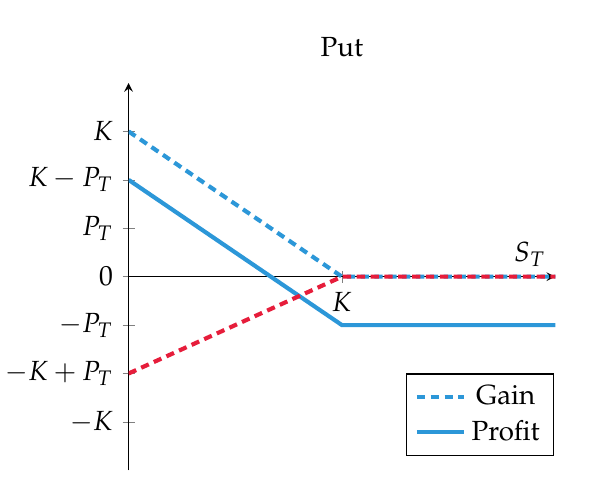
\begin{tikzpicture}
    \hspace{-4mm}
    \begin{axis}[
        height=6.5cm,
        width=7cm,
        axis x line=middle,
        axis y line=left,
        xlabel={$S_T$},
        xtick={1},
        xticklabels={$K$},
        ytick={1.5,1,  0.5,0, -0.5, -1,  -1.5},
        yticklabels={$K$ , $K - P_T$, $P_T$,0,$-P_{T}$,$-K + P_T$, $-K$},
        title={Put},
        legend entries={Gain,Profit},
        legend style={at={(0.65,0.25)},anchor=north west},
        xmin = 0,
        xmax = 2,
        ymin = -2,
        ymax = 2]
        % payoff sur position short
        \addplot[mark=none, draw=ShortColor, line width=1.5pt, densely dashed] coordinates { (0,1.5) (1,0) (2,0) };
        % profit sur position short
        \addplot[mark=none, draw=ShortColor, line width=1.5pt] coordinates { (0,1) (1,-0.5) (2,-0.5) };
        % payoff sur position long
        \addplot[mark=none, draw=LongColor, line width=1.5pt, densely dashed] coordinates { (0, -1) (1,0) (2,0) };
    \end{axis}
\end{tikzpicture}

\section*{Stratégies de couverture de base}

\subsection*{Floor}
\begin{itemize}
\item \emph{long stock}
\item \emph{short put} (i.e. on achète une option de vente)
\end{itemize}

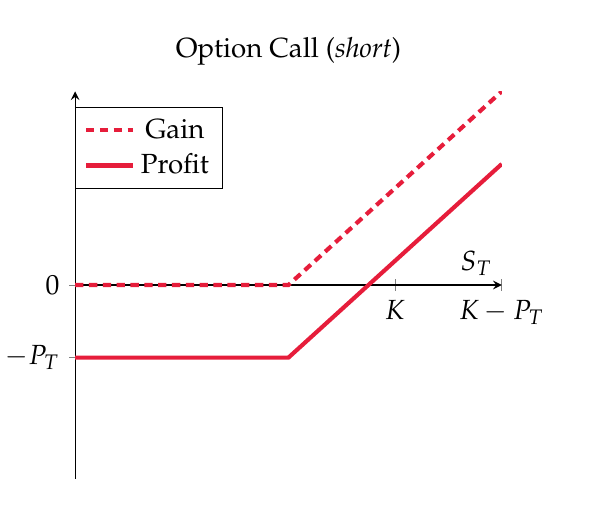
\begin{tikzpicture}
    \hspace{-4mm}
    \begin{axis}[
        height=6.5cm,
        width=7cm,
        axis x line=middle,
        axis y line=left,
        xlabel={$S_T$},
        xtick={1.5, 2},
        xticklabels={$K$, $K - P_T$},
        ytick={0, -0.75},
        yticklabels={0,$-P_{T}$},
        title={Option Call (\emph{short})},
        legend entries={Gain,Profit},
        legend style={at={(0,0.96)},anchor=north west},
        xmin = 0,
        xmax = 2,
        ymin = -2,
        ymax = 2]
        \addplot[mark=none, draw=LongColor, line width=1.5pt, densely dashed] coordinates { (0,0) (1,0) (2,2) };
        \addplot[mark=none, draw=LongColor, line width=1.5pt] coordinates { (0,-0.75) (1,-0.75) (2,1.25) };
    \end{axis}
\end{tikzpicture}







\end{multicols*}

%% -----------------------------
%% Fin du document
%% -----------------------------
\end{document}